\chapter{\textit{Frameworks} MVC e de Persistência}\label{cap:frameworksPersistencia}
\epigraph{``\textit{A persistência é o caminho do êxito}''.}{Charles Chaplin}
\epigraph{``\textit{Não extingua sua inspiração e sua imaginação; não se torne o escravo do seu modelo}''.}{Vincent van Gogh}

\lettrine[lines=4, lhang=0.1, lraise=0, loversize=0.2, findent=0.1em]{\textcolor{corTema}{N}}{ESTE} Capítulo reconstruiremos o ``Sistema de Venda de Produtos'' do Capítulo~\ref{cap:terceiroProjeto} utilizando diversos \textit{frameworks} que tornarão nosso trabalho menos tedioso e mais direto ao ponto!

\vfill

\section{Introdução}

Antes de começarmos a trabalhar, precisamos configurar nosso ambiente de desenvolvimento. Como lidaremos com toda a \textit{stack} de \textit{frameworks} e bibliotecas do Spring, poderíamos utilizar a ferramenta oficial deles para nos auxiliar, a Spring Tool Suite 4. Eu particularmente não sou muito fã, pois ela é baseada na IDE Eclipse que, na minha opinião, é extremamente burocrática e instável, mas como ela é adotada como o padrão da indústria, uma hora ou outra acabamos ter que a adotar. Continuaremos a utilizar o NetBeans como nossa ferramenta padrão, mas você pode testar a Spring Tool Suite caso deseje. No momento em que este texto está sendo escrito existem também versões para o Visual Studio Code (\url{https://code.visualstudio.com/}) a para a IDE Theia (\url{https://theia-ide.org/}). O download de qualquer uma das versões pode ser feito em \url{https://spring.io/tools}.

A primeira coisa que vamos fazer é acessar o site Spring Initializr (\url{https://start.spring.io/}). Nesse site podermos configurar a infraestrutura básica do nosso projeto, que utilizará o Maven (\url{https://maven.apache.org/}) como ferrameta de gerenciamento do projeto. O Maven é suportado atualmente pelas principais IDEs disponíveis. Sendo um projeto Maven, espera-se que todas as IDEs trabalhem de forma semelhante, então teoriacemente podemos trabalhar com mais de uma ferramenta no mesmo projeto. Note que iremos reconstruir o ``Sistema de Venda de Produtos'' do Capítulo\ref{cap:terceiroProjeto}. Vamos começar?

A versão atual da página principal do site do Spring Initializr pode ser vista na Figura~\ref{fig:cap10SpringInitializr}.

\FloatBarrier
\begin{figure}[!htbp]
    \centering
    \caption{Tela principal do site do Spring Initializr}
    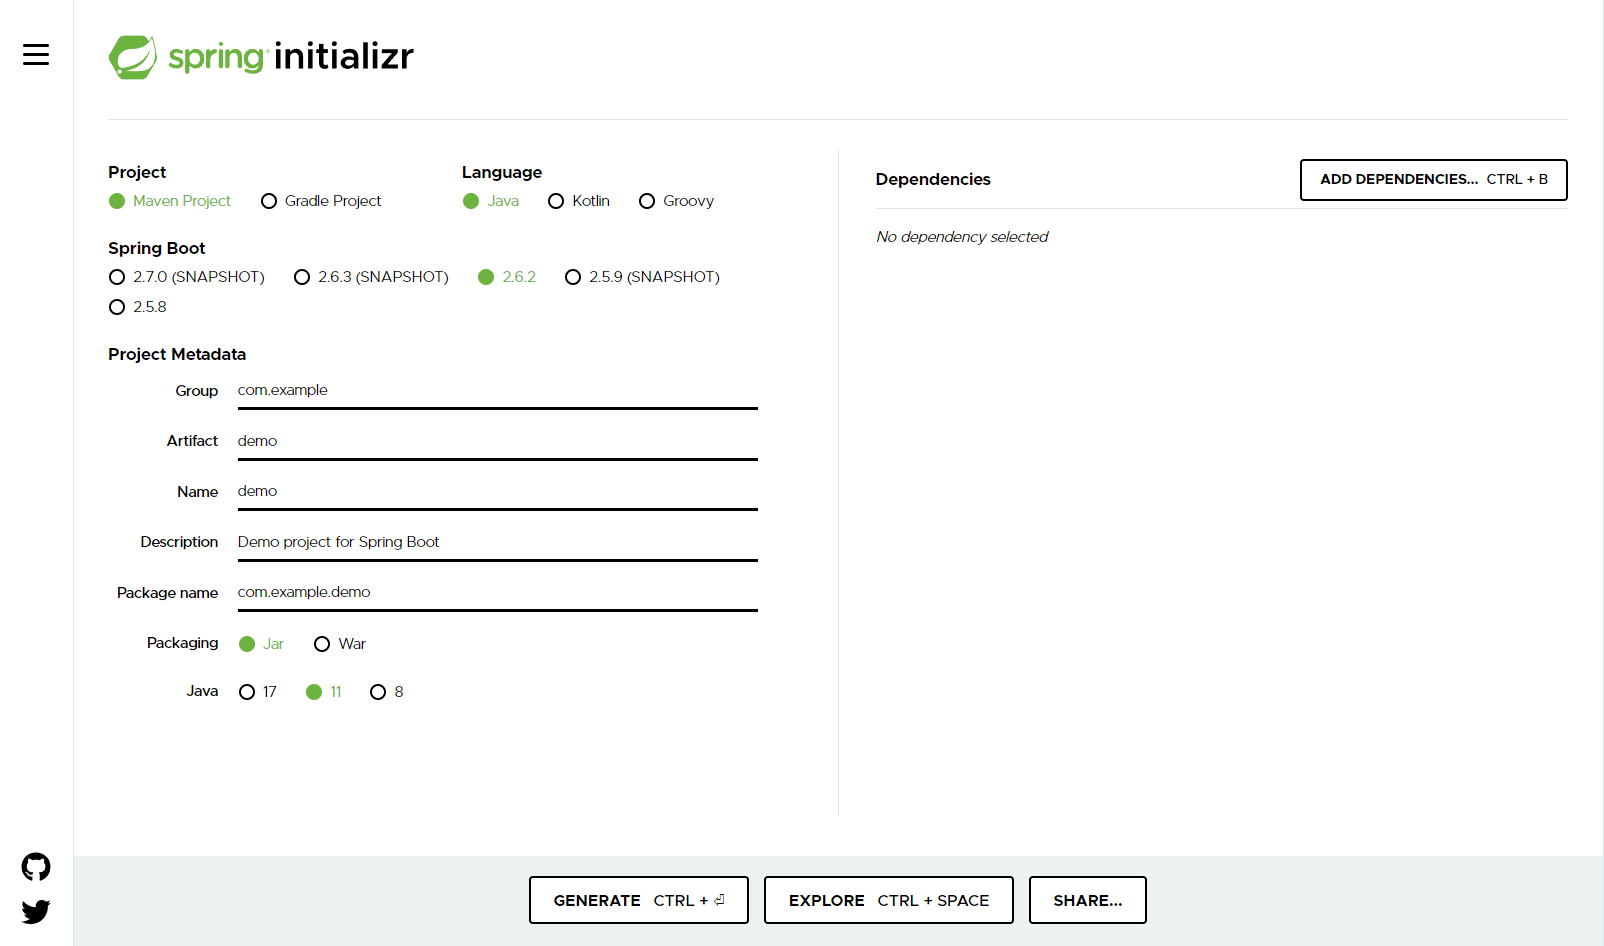
\includegraphics[scale=0.4]{imagens/cap10SpringInitializr}
    \\\textbf{Fonte:} \url{https://start.spring.io/}
    \label{fig:cap10SpringInitializr}
\end{figure}
\FloatBarrier

Basicamente do lado esquerdo temos as opções de configuração do projeto:
\begin{itemize}
    \item \textbf{Project:} qual ferramenta de gerencimanto de projeto será usada;
    \item \textbf{Language:} a linguagem de programação do projeto;
    \item \textbf{Spring Boot:} qual a versão do Spring Boot que usaremos;
    \item \textbf{Project Metadata:} os metadados do projeto:
    \begin{itemize}
    content...
    \end{itemize}
    \item \textbf{:}
    \item \textbf{:}
    \item \textbf{:}
    \item \textbf{:}
    \item \textbf{:}
    \item \textbf{:}
\end{itemize}

\FloatBarrier
\begin{figure}[!htbp]
    \centering
    \caption{Definição das propriedades do Projeto}
    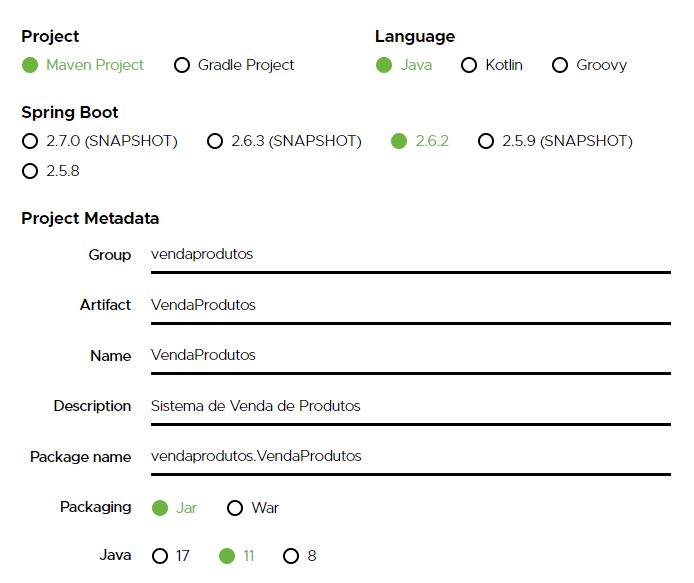
\includegraphics[scale=0.7]{imagens/cap10SpringInitializrConfProjeto01}
    \\\textbf{Fonte:} \url{https://start.spring.io/}
    \label{fig:cap10SpringInitializrConfProjeto01}
\end{figure}
\FloatBarrier

\begin{itemize}
    \item \textbf{Spring Boot DevTools:} auxília no desenvolvimento de aplicações usando Spring Boot;
    \item \textbf{Spring Framework:} \textit{framework} que possibilita a injeção de dependências e a inversão de controle;
    \item \textbf{Spring Data JPA:} \textit{framework} para persistência de dados usando Hibernate e a Java Persistence API (JPA);
    \item \textbf{Spring Validation:} permite a validação de objetos que serão gerenciados pela aplicação (já fizemos algo parecido);
    \item \textbf{Spring Web:} construção de aplicações Web usando o padrão de projeto MVC através do \textit{framework} Spring MVC, além da criação de Web Services RESTful;
    \item \textbf{Lombok:} é uma biblioteca de anotações que nos ajuda na criação automática de código padronizado como getters, setters, construtores etc;
    \item \textbf{Thymeleaf:} é uma \textit{template engine} que permite a definição de modelos para a criação de interfaces gráficas usando HTML, diminuindo a duplicidade de código e facilitando a manutenção do código.
\end{itemize}

\FloatBarrier
\begin{figure}[!htbp]
    \centering
    \caption{Definição das dependências do projeto}
    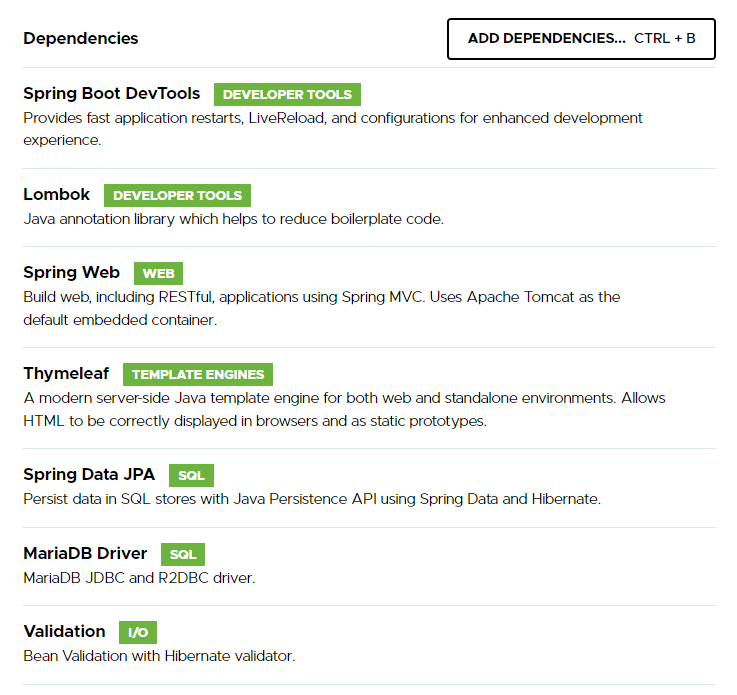
\includegraphics[scale=0.7]{imagens/cap10SpringInitializrConfProjeto02}
    \\\textbf{Fonte:} \url{https://start.spring.io/}
    \label{fig:cap10SpringInitializrConfProjeto02}
\end{figure}
\FloatBarrier

Agora com o inicializador do projeto configurado, clique no botão ``GENERATE''. Ao fazer isso, um arquivo .zip será baixado. No local onde foi salvo, descompacte-o. Abra o NetBeanse realize o procedimento de abrir projetos. Vá à pasta onde o arquivo zip foi descompactado. Você notará que o NetBeans reconhecerá um projeto Maven ali. Selecione-o e abra-o.

Note que se você quiser, pode usar o \textit{link} abaixo para fazer o \textit{download} do projeto com as mesmas configurações apresentadas.

\url{https://start.spring.io/#!type=maven-project&language=java&platformVersion=2.6.2&packaging=jar&jvmVersion=11&groupId=vendaprodutos&artifactId=VendaProdutos&name=VendaProdutos&description=Sistema%20de%20Venda%20de%20Produtos&packageName=vendaprodutos.VendaProdutos&dependencies=devtools,lombok,web,thymeleaf,data-jpa,mariadb,validation}

Provavelmente, após abrir o projeto, seu NetBeans vai demorar alguns minutos --pode demorar bastante na verdade-- para baixar o índice central do Maven e prepará-lo no seu computador. Após esse processo, seu NetBeans vai ``reclamar'', informando que o projeto não contém as dependências no repositório local do Maven. Veja na Figura~\ref{fig:cap10ConfProjeto03} o que provavelmente aparecerá, ou seja, um sinal de aviso (\textit{warning}) no ícone do projeto.

\FloatBarrier
\begin{figure}[!htbp]
    \centering
    \caption{Resolução de problema do projeto criado}
    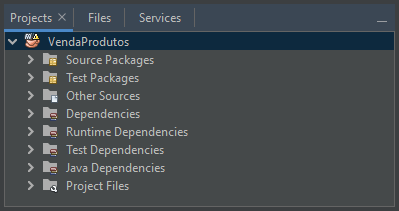
\includegraphics[scale=1]{imagens/cap10ConfProjeto03}
    \\\textbf{Fonte:} Elaborada pelo autor
    \label{fig:cap10ConfProjeto03}
\end{figure}
\FloatBarrier

Para resolvermos isso, faremos algo que talvez você já tenha feito para outras situações. Clique com o botão direito no projeto e escola a opção \destaque{\textit{Resolve Project Problems...}} do menu de contexto. Fazendo isso, um diálogo aparecerá com um ou mais itens com o texto ``\textit{Some dependency artifacts are not in the local repository}'', indicando o problema encontrado. Clique no botão \destaque{\textit{``Resolve''}}. O Maven vai começar a realizar o processo de ``Priming'' (preparação) do projeto, prepararando e baixando todas as dependências. Essa preparação pode demorar um pouco também. Você saberá que o processo terminou quando aparecer ``BUILD SUCESS'' na saída do NetBeans e quando o diálogo da solução dos problemas do projeto apresentar o problema apontado anteriormente com um ``check'' ou ``tick'' verde. Clique em Close.

explicar estrutura do projeto

falar  other sources para mostrar como diretórios

rodar pela primeira vez

criar um index

configurar o WebConfig

como executar

como associar ao navegador com LiveReload

arquivo de configurações do Spring Boot

falar do POM


\section{Hibernate, JPA, Validações e Lombok}

criação das entidades
carga inicial no banco


\section{Spring MVC}

criação dos controladores e páginas com thymeleaf


\subsection{Outros \textit{Frameworks} MVC}

%Falar brevemente de: JavaServer Faces (JSF), Struts, VRaptor etc.


\section{\textit{Web Services RESTful}}

criação de controladores rest e consumir API usando Javascript.

talvez uma inserção e uma listagem?


\section{Resumo}

\section{Exercícios}

\section{Projetos}
